%!TEX program = xelatex
\documentclass[UTF8]{ctexart}

\setmainfont{Times New Roman}
\setCJKmainfont{宋体}
% math bracket
%  ()
\newcommand{\brc}[1]{\left({{}#1}\right)}
%  []
\newcommand{\brm}[1]{\left[{{}#1}\right]}
%  ||
\newcommand{\brv}[1]{\left|{{}#1}\right|}
%  {}
\newcommand{\brf}[1]{\left\{{{}#1}\right\}}
%  ||
\newcommand{\brt}[1]{\left\Vert{{}#1}\right\Vert}
%  <>
\newcommand{\brg}[1]{\left<{{}#1}\right>}
%  floor
\newcommand{\floor}[1]{\lfloor{{}#1}\rfloor}
%  ceil
\newcommand{\ceil}[1]{\lceil{{}#1}\rceil}

% font
\newcommand{\fira}[1]{{\firacode {}#1}}

% abbr command
\newcommand{\ds}{\displaystyle}
\newcommand{\pt}{\partial}
\newcommand{\rint}[2]{\Big|^{{}#1}_{{}#2}}
\newcommand{\leg}{\left\lgroup}
\newcommand{\rig}{\right\rgroup}

% math symbol
\newcommand{\de}{\mathrm{d}}
\newcommand{\im}{\mathrm{im}}
\newcommand{\ord}{\mathrm{ord}}
\newcommand{\cov}{\mathrm{Cov}}
\newcommand{\lub}{\mathrm{LUB}}
\newcommand{\glb}{\mathrm{GLB}}
\newcommand{\var}{\mathrm{Var}}
\newcommand{\aut}{\mathrm{Aut}}
\newcommand{\sylow}{\mathrm{Sylow}}
\newcommand{\xhi}{\mathcal{X}}
\newcommand{\po}{\mathcal{P}}
\newcommand{\bi}{\mathrm{b}}
\newcommand{\rfl}{\mathcal{R}}

% algorithmic symbol
\newcommand{\gro}{\mathrm{O}}

% control command
\newcommand{\hfindent}{\hspace*{1em}}

\newfontfamily\firacode{Fira Code}
\newfontfamily\mincho{MS Mincho}

% math
\usepackage{ntheorem}
\usepackage{ulem}

\theoremseparator{ }
\newtheorem{dft}{Definition}
\newtheorem{tem}[dft]{Theorem}
\newtheorem{lem}[dft]{Lemma}
\newtheorem{epe}[dft]{Example}
\newtheorem{cor}[dft]{Corollary}

\usepackage{mathrsfs}
\usepackage{amsmath}
\usepackage{amssymb}
\usepackage{cancel}
%\usepackage{amsthm}

% control
\usepackage{ifthen}
\usepackage{intcalc}
\usepackage{array}

% format
\usepackage{indentfirst}
\usepackage{enumerate}
\usepackage{url}
\usepackage{setspace}

\usepackage{xcolor}

\definecolor{ballblue}{rgb}{0.13, 0.67, 0.8}
\definecolor{celestialblue}{rgb}{0.29, 0.59, 0.82}
\definecolor{bananayellow}{rgb}{1.0, 0.88, 0.21}
\definecolor{brilliantlavender}{rgb}{0.96, 0.73, 1.0}
\definecolor{burgundy}{rgb}{0.5, 0.0, 0.13}
\definecolor{cadmiumorange}{rgb}{0.93, 0.53, 0.18}
\definecolor{aqua}{rgb}{0.0, 1.0, 1.0}
\definecolor{auburn}{rgb}{0.43, 0.21, 0.1}
\definecolor{brass}{rgb}{0.71, 0.65, 0.26}
\definecolor{tangerine}{rgb}{0.95, 0.52, 0.0}
\definecolor{portlandorange}{rgb}{1.0, 0.35, 0.21}
\definecolor{mediumred-violet}{rgb}{0.73, 0.2, 0.52}
\definecolor{darkpastelpurple}{rgb}{0.59, 0.44, 0.84}

% listing set
\definecolor{func}{rgb}{0.29, 0.59, 0.82}
\definecolor{ftype}{rgb}{0.59, 0.44, 0.84}
\definecolor{cls}{rgb}{1.0, 0.35, 0.21}
\definecolor{slf}{rgb}{0.73, 0.2, 0.52}
\definecolor{backg}{HTML}{F7F7F7}
\definecolor{str}{HTML}{228B22}
% attestation
\definecolor{atte}{RGB}{178,34,34}

\usepackage{listings}

\lstset{
    backgroundcolor = \color{backg},
    basicstyle = \small,%
    escapeinside = ``,%
    keywordstyle = \color{func},% \underbar,%
    identifierstyle = {},%
    commentstyle = \color{blue},%
    stringstyle = \color{str}\ttfamily,%
    %labelstyle = \tiny,%
    extendedchars = false,%
    linewidth = \textwidth,%
}

\usepackage{geometry}

\geometry{
    left=2.0cm,
    right=2.0cm,
    top=2.5cm,
    bottom=2.5cm
}

\usepackage[
    colorlinks,
    linkcolor=blue,
    anchorcolor=blue,
    citecolor=blue
]{hyperref}

% table
\usepackage{csvsimple}
\usepackage{multirow}

% picture
\usepackage{graphicx}


% graph
\usepackage{tikz}
\usepackage{pgfplots}
\usetikzlibrary{
    quotes,
    angles,
    matrix,
    arrows,
    automata
}


\title{Tango v3.2.0文档}
\author{Myriad-Dreamin 2017211279 2017211301}
\date{}

\begin{document}
\setlength{\parindent}{2em}
%\renewcommand{\baselinestretch}{1.5}
\setlength{\baselineskip}{2.5em}
\maketitle
所有版本的github托管网站:\url{https://github.com/Myriad-Dreamin/Tango}
\section{Tango架构}
\subsection{服务器端-客户端架构}
Tango采用服务器端-客户端架构。两者使用公共的TangoLib(TangoCommon)库。
在TangoCommon中目前一共包含六大内容。\\
\hfindent\textbf{automator}\\
\indent automator中包含两大类,一是GameAutomation, 二是GameConfig.\\
\indent GameAutomation共同的基类是AbstractGameAutomation,GameAutomation真正实现了游戏的逻辑,而GameAutomationRelayer仅仅拥有一个信号转发机制。\\
\indent GameAutomation依赖的一个类是GameConfig.GameConfig中包含了各种游戏的设置,例如经验更新,例如回答时间的计算,例如当前游戏的单词池。\\
\hfindent\textbf{client}\\
\indent client中只有一种类,即Client类。Client类都有一个共同的抽象基类AbstractClient,其下有三个类。\\
\indent LocalClient负责完成与本地数据库交互的逻辑,RemoteClient负责完成与远程服务器交互的逻辑,Client负责完成LocalClient或者RemoteClient与客户端图形化界面的配接。\\
\hfindent\textbf{component}\\
\indent component中包含一些常用的组件。Logger是分级的日志管理,MessageBox是适用于客户端的特殊的消息框,PairTableItem用于一些组合型的Widget场景,TimerWidget是一个用于显示可倒计时的特殊Wdiget。\\
\hfindent\textbf{network}\\
\indent network中包含服务器端和客户端共享的一套网络协议。SocketX为QTcpSocket的子类,在QTckSocket的基础上约定了包发送和接受的处理。client\_rpc是客户端和服务器端收发消息遵守的一套json\_rpc协议。\\
\hfindent\textbf{players}\\
\indent players中包含一大类,Player是Consumer和Author的共同基类。Player中包含与数据库交互的底层逻辑和自身所带的属性信息。\\
\hfindent\textbf{types}\\
\indent typers是杂类,包含一系列有意义的枚举常量(enumeration)或者命名元组(named tuple)。\\
\subsection{Tango库}
\begin{enumerate}[1]
    \item \textcolor{cls}{Class} automator/AbstractGameAutomation 抽象自动机类
    \item \textcolor{cls}{Class} automator/AbstractGameAutomation.GameAutomation 自动机类
    \item \textcolor{cls}{Class} automator/AbstractGameAutomation.GameAutomationRelayer 转接自动机类
    \item \textcolor{cls}{Class} automator/GameConfig 游戏设定类
    \item \textcolor{cls}{Class} client/AbstractClient 抽象客户端类
    \item \textcolor{cls}{Class} client/AbstractClient.LocalClient 本地客户端类
    \item \textcolor{cls}{Class} client/AbstractClient.RemoteClient 远程客户端类
    \item \textcolor{cls}{Class} client/AbstractClient.Client 客户端类
    \item \textcolor{cls}{Class} component/Logger 日志类
    \item \textcolor{cls}{Class} component/MessageBox 消息框类
    \item \textcolor{cls}{Class} component/PairTableItem 表对类
    \item \textcolor{cls}{Class} component/TimerWidget 计时器类
    \item \textcolor{func}{Library} network/client\_rpc 消息rpc库
    \item \textcolor{cls}{Class} network/SocketX TangoSocket类
    \item \textcolor{cls}{Class} players/Player 玩家类
    \item \textcolor{cls}{Class} players/Author 作者类
    \item \textcolor{cls}{Class} players/Consumer 读者类
    \item \textcolor{str}{Enum} types/RetriveMode 数据库Fetch模式枚举类型
    \item \textcolor{cls}{Class} types/TangoPair 单词类
    \item \textcolor{cls}{Class} types/UserBriefInfo 简略用户信息类
    \item \textcolor{cls}{Class} types/UserFullInfo 详细用户信息类
    \item \textcolor{str}{Enum} types/UserStatus 用户状态枚举类型
\end{enumerate}
\subsection{客户端}
\begin{enumerate}[1]
    \item \textcolor{func}{Function} main 主程序入口
    \item \textcolor{cls}{Class} MainWindow 窗口类
    \item \textcolor{cls}{Class} Scene 场景类
    \item \textcolor{cls}{Class} Scene.CreationScene
    \item \textcolor{cls}{Class} Scene.MainScene
    \item \textcolor{cls}{Class} Scene.MultiplayScene
    \item \textcolor{cls}{Class} Scene.PlayingScene
    \item \textcolor{cls}{Class} Scene.PlaySettleScene
    \item \textcolor{cls}{Class} Scene.PlaySubScene
    \item \textcolor{cls}{Class} Scene.QueryUsersScene
    \item \textcolor{cls}{Class} Scene.RankingAuthorsScene
    \item \textcolor{cls}{Class} Scene.RankingConsumersScene
    \item \textcolor{cls}{Class} Scene.RegisterScene
    \item \textcolor{cls}{Class} Scene.SelectingScene
\end{enumerate}
\subsection{服务端}
\begin{enumerate}[1]
    \item \textcolor{func}{Function} main 主程序入口
    \item \textcolor{cls}{Class} MainWindow 窗口类
    \item \textcolor{cls}{Class} engine/TcpServer 服务器类
    \item \textcolor{cls}{Class} engine/TangoThread 服务器线程类
\end{enumerate}
\section{核心逻辑}
\subsection{Client转接逻辑}
LocalClient和RemoteClient都是AbstractClient的子类。MainWindow(客户端)不关心LocalClient和RemoteClient具体实现,仅仅是利用了Client类的\fira{setup\_remote\_connection}或是\fira{setup\_local\_connection}申请touch Model。
\begin{figure}[!h]
    \centering
    \begin{tikzpicture}[->,>=stealth',shorten >=1pt,auto,node distance=2.8cm,semithick]
    \tikzstyle{every state}=[shape=rectangle, rounded corners]
    \node[state] (main) at (0, 0){MainWindow};
    \node[state] (c) at (4, 0){Client};
    \node[state] (l) at (8.5, 1){LocalClient};
    \node[state] (r) at (8.5, -1){RemoteClient};
    \node[state] (b) at (12, 1){Mysql Service};
    \node[state] (s) at (12, -1){TangoServer};
    \node[rotate = 350] at (5.9, -0.5) {远程连接};
    \node[rotate = 10] at (5.9, 0.5) {本地连接};
    \path (main) edge [out=0, in=180] node{请求连接} (c);
    \path (c) edge [out=0, in=200] (l);
    \path (c) edge [out=0, in=160] (r);
    \path (l) edge [out=0, in=180] node{连接} (b);
    \path (r) edge [out=0, in=180] node{连接} (s);
    \end{tikzpicture}
    \caption{Client转接逻辑(连接)}
\end{figure}\\
\indent 申请服务时,TangoServer实际上也使用LocalClient与服务器上的Mysql服务交互。\\
\begin{figure}[!h]
    \centering
    \begin{tikzpicture}[->,>=stealth',shorten >=1pt,auto,node distance=2.8cm,semithick]
    \tikzstyle{every state}=[shape=rectangle, rounded corners]
    \node[state] (main) at (0, 0){MainWindow};
    \node[state] (c) at (4, 0){Client};
    \node[state] (l) at (9, 1){Native Mysql Service A};
    \node[state] (r) at (8.5, -1){TangoServer};
    \node[state] (s) at (14, -1){Remote Mysql Service B};
    \node[rotate = 350] at (5.9, -0.5) {RemoteClient};
    \node[rotate = 10] at (5.9, 0.5) {LocalClient};
    \path (main) edge [<->, out=0, in=180] node{请求数据} node[below]{返回数据} (c);
    \path (c) edge [out=0, in=195] (l);
    \path (c) edge [<->, out=0, in=160] (r);
    \path (r) edge [<->, out=0, in=180] node{LocalClient} (s);
    \end{tikzpicture}
    \caption{Client转接逻辑(请求数据)}
\end{figure}\\
\indent 事实上,由于Client的设计,TangoServer可以是一个子服务器,继续转接母服务器。
\subsection{游戏逻辑}
\subsubsection{MainWindow向Client请求游戏服务}
GameAutomation(简称GA)和GameAutomationRelayer(简称GAR)都是AbstractGameAutomationRelayer(简称AGA)的子类。\\
\begin{figure}[!h]
    \centering
    \begin{tikzpicture}[->,>=stealth',shorten >=1pt,auto,node distance=2.8cm,semithick]
    \tikzstyle{every state}=[shape=rectangle, rounded corners]
    \node[state] (main) at (0.3, 0){MainWindow};
    \node[state] (c) at (4, 0){Client};
    \node[state] (l) at (8.5, 1){LocalClient};
    \node[state] (r) at (8.5, -1){RemoteClient};
    \node[state] (b) at (13, 1){Mysql Service};
    \node[state] (s) at (13, -1){TangoServer};
    \node[state] (g) at (15.8, -1){GA};
    \node[rotate = 350] at (5.9, -0.5) {远程服务};
    \node[rotate = 10] at (5.9, 0.5) {本地服务};
    \path (main) edge [out=0, in=180] node{请求游戏} (c);
    \path (c) edge [out=0, in=200] (l);
    \path (c) edge [out=0, in=160] (r);
    \path (l) edge [out=0, in=180] node{请求单词} (b);
    \path (r) edge [out=0, in=180] node{请求服务} (s);
    \path (s) edge [out=0, in=180] node{创建} (g);
    \end{tikzpicture}
    \caption{MainWindow请求游戏(请求)}
\end{figure}\\
MainWindow从Client请求到的是AGA的handler,根据AGA发出的信号做出动作。
\begin{figure}[!h]
    \centering
    \begin{tikzpicture}[->,>=stealth',shorten >=1pt,auto,node distance=2.8cm,semithick]
    \tikzstyle{every state}=[shape=rectangle, rounded corners]
    \node[state] (main) at (0, 0){MainWindow};
    \node[state] (c) at (4, 0){Client};
    \node[state] (l) at (8.5, 1){LocalClient};
    \node[state] (r) at (8.5, -1){RemoteClient};
    \node[state] (b) at (12, 1){Mysql Service};
    \node[state] (s) at (12.5, -1){TangoServer};
    \node[state] (g) at (15.7, -1){GA};
    \node[rotate = 350] at (5.9, -0.5) {GAR};
    \node[rotate = 10] at (5.9, 0.5) {GA};
    \path (main) edge [<-, out=0, in=180] node{AGA} (c);
    \path (c) edge [<-, out=0, in=200] (l);
    \path (c) edge [<-, out=0, in=160] (r);
    \path (l) edge [<-, out=0, in=180] node{单词} (b);
    \path (r) edge [<-, out=0, in=180] node{signals} (s);
    \path (s) edge [<-, out=0, in=180] node{signals} (g);
    \end{tikzpicture}
    \caption{MainWindow请求游戏(返回handler)}
\end{figure}
\subsubsection{AGA信号发射}
\begin{figure}[!h]
    \centering
    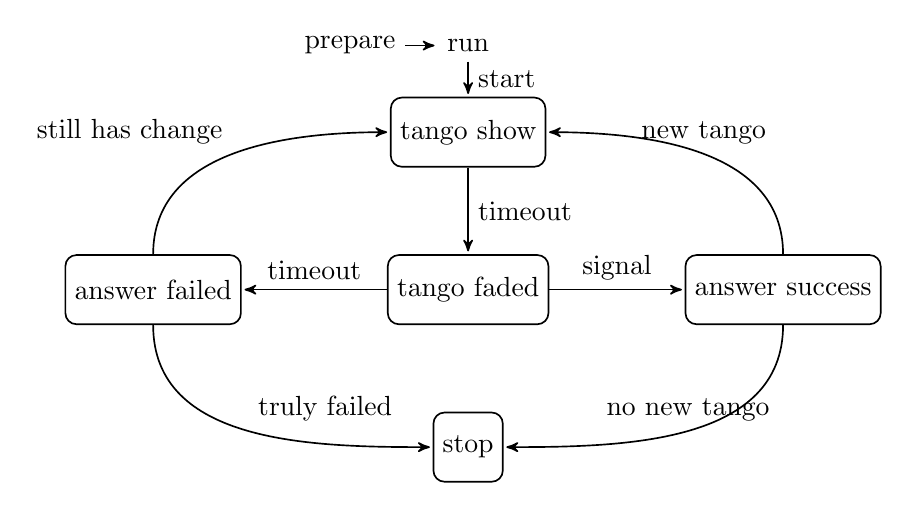
\begin{tikzpicture}[->,>=stealth',shorten >=1pt,auto,node distance=2.8cm,semithick]
    \tikzstyle{every state}=[shape=rectangle, rounded corners]
    \node (p) at (0, 0.1) {prepare};
    \node (r) at (1.5, 0.1) {run};
    \node[state] (nt) at (1.5, -1) {tango show};
    \node[state] (tf) at (1.5, -3) {tango faded};
    \node[state] (as) at (5.5, -3) {answer success};
    \node[state] (af) at (-2.5, -3) {answer failed};
    \node[state] (st) at (1.5, -5) {stop};
    \path (p) edge [out=0, in=180] (r);
    \path (r) edge [out=270, in=90] node{start} (nt);
    \path (nt) edge [out=270, in=90] node{timeout} (tf);
    \path (tf) edge node{signal} (as);
    \path (tf) edge node [above] {timeout} (af);
    \path (af) edge [out=270, in=180] node{truly failed} (st);
    \path (as) edge [out=270, in=0] node[above]{no new tango} (st);
    \path (af) edge [out=90, in=180] node{still has change} (nt);
    \path (as) edge [out=90, in=0] node[above]{new tango} (nt);
    \end{tikzpicture}
    $$
    \begin{matrix}
        g(\text{tango show}, \text{tango faded}) = \text{new tango}, \text{fade time}\\
        g(\text{tango faded}, \text{answer failed}) = \text{tango faded}, \text{answer time}\\
        g(\text{tango faded}, \text{answer success}) = \text{tango faded}, \text{answer time}\\
        g(\text{answer failed}, \text{stop}) = \text{failed},
        g(\text{answer success}, \text{stop}) = \text{success}\\
    \end{matrix}
    $$
    \caption{GA自动机}
\end{figure}
MainWindow就是根据这个自动机的输出完成一系列的游戏动作。
\subsubsection{GameConfig的功能}
GameConfig允许定制下面几个参量:
\begin{enumerate}[\indent\indent 1]
    \item 每次显示单词的定时器时间变化
    \item 每次回答单词的定时器时间变化
    \item 每次回答失败是否真的失败的选项
    \item 每次单词回答成功经验如何变化
    \item 初始的显示单词的定时器时间
    \item 初始的回答单词的定时器时间
    \item 单词缓存是否独立
\end{enumerate}
前四个选项分别需要传入四个函数指针.
{\firacode
\begin{lstlisting}[language={[ANSI]C}]
    /* 消失时间变换函子, 每次单词作答完以后作用一次 */
    std::function<void(int&)> fade_functor;
    /* 回答时间变换函子, 每次单词作答完以后作用一次 */
    std::function<void(int&)> ans_functor;
    /* 经验计算函子, 传入一个单词和当前轮数作为参考 */
    std::function<void(int&,TangoPair,int)> exp_functor;
    /* 每次失败事件触发以后, 调用失败函数函子判断是否仍有机会 */
    std::function<bool()> if_failed_functor;
\end{lstlisting}
}
例如默认的经验值函数子为:
{\firacode
\begin{lstlisting}[language={[ANSI]C}]
    void default_exp_functor(int &x, TangoPair tango, int)
    {
        x += tango.first.length();
        return;
    }
\end{lstlisting}
}
这个经验值函数选择将单词的长度作为经验值增加。当我们切换游戏模式为困难模式时。
{\firacode
\begin{lstlisting}[language={[ANSI]C}]
    void hard_exp_increment(int &exp, TangoPair tango, int success_count)
    {
        exp = exp + static_cast<int>(
            tango.first.length() * (1.4 + success_count * 0.03) + 0.99
        );
    }
\end{lstlisting}
}
直接修改这个函数为一个更快非线性的增长即可。\\
\indent GA接受一个GameConfig参数构造,每次在特定的时刻调用Config中的函子或者使用其中的参量。\\
\indent 以此为基础,本文设置了四个不同的难度和经验等级,四个不同的单词选取模式,一共16种组合,并在难度较大的情况下,让玩家拥有多次复活重新答题的机会(斟酌给了一次)。\\
\indent 如此看来,将GA和GameConfig解构,确实是一个不错的选择。
\subsection{MainWindow在客户端中的功能层次}
MainWindow将每个不同的界面组织为场景。将自己身为客户端界面的主动承担者化为被动服务者。MainWindow将CenterWidget让诸场景类,只提供与Client的交互或其他长期存在的全局服务。\\
\indent MainWindow现在仅有一个供使用的函数\fira{switch scene},用于切换CenterWidget内含的场景实例.
\indent 当进入场景时, MainWindow会调用scene的\fira{on\_incoming}无状态函数,当离开场景时,MainWindow会调用scene的\fira{on\_exiting}无状态函数。
\subsection{重新设计传输层协议}
在QT自带的TcpSocket传输层的基础上,本文添加了新的传输层协议功能。\\
\begin{figure}[!h]
    \centering
    \begin{tikzpicture}[->,>=stealth',shorten >=1pt,auto,node distance=2.8cm,semithick]
    \tikzstyle{every state}=[shape=rectangle, rounded corners]
    \node[state] (a) at (0,0) {ENTITY-A};
    \node[state] (sxa) at (0,-1.5) {SocketX};
    \node[state] (b) at (4,0) {ENTITY-B};
    \node[state] (sxb) at (4,-1.5) {SocketX};
    \draw[rounded corners] (-2, -3.5) rectangle (6, -2.5);
    \node (tcp) at (2,-3) {TcpSocket};
    \draw[->] (0, -0.5) -- node[left]{发包} (0, -1);
    \draw[<-] (4, -0.5) -- node[left]{取包} (4, -1);
    \draw[->] (0, -2) -- node[left]{加密} (0, -2.5);
    \draw[<-] (4, -2) -- node[left]{解密} (4, -2.5);
    \end{tikzpicture}
    \caption{包的传输流}
\end{figure}\\
\indent SocketX使用Base64可逆的功能性加密算法,避免不可见字符代表的字节出现在字节流中,并约定一个包界限符(如SocketX使用的0x1字节),完成无需等待的异步请求和响应。这种协议的好处是,既拥有线性的时间复杂度(Base64的时空代价极小),可靠的服务(TCP)特性,又拥有报文式请求特性。
\subsection{使用json-rpc网络服务}
关于json-rpc的详细内容,这里不做介绍。json-rpc就是以json字节流服务为基础的rpc远程请求服务。本文前面举例的远程服务,将json-rpc的无状态服务以约定的方式,完成了服务器端与客户端的同步行为。所谓约定的方式,就是双方约定共同的函数编号,游戏设置编号,信息交换请求。
\subsection{难度和等级计算公式举例}
以初级难度为例。Fetch模式为为在长度区间在[0\%, 80\%]比例的单词中随机选取连续的N段。回答时间随着单词个数增加每次减少50ms,至少保证1s的单词显示时间。经验见计算公式。
$$
    atime=\text{dfunc}(x)=\max\{1000, x-50\}ms, exp=\sum_{i}\floor{ length[tango[i]] * (1 + i * 0.01) + 0.99}
$$
\subsection{自定义日志管理}
QT的日志管理还是很原始的。因此我重写了一个通用的C++日志管理。\\
\indent Logger支持5级日志分级管理,支持单例日志申请。暂时不支持支持多线程,不支持自定义文件输出。日志类全程采用type traits特性和模板元百编程,因此任意信息进入日志只需要一级转移,速度非常快。
\section{v3基础功能}
主界面如图六,比较土。\\
\begin{figure}[h]
    \centering
    \includegraphics[scale=0.3]{./images/main_view.png}
    \caption{主界面}
\end{figure}\\
\indent 点击登录按钮进入登录界面,点击注册按钮进入注册界面,点击设置按钮进入设置界面,点击退出按钮退出游戏。设置界面是v3.2新加入的功能。\\
\indent 登录界面如图七。远程连接是初期定下的功能,将来会移动至设置界面。远程连接的checkbox被按下时,选择远程连接,否则选择本地连接服务。\\
\indent 输入正确用户名和密码进入游玩界面。\\
\begin{figure}[!ht]
    \centering
    \includegraphics[scale=0.3]{./images/login_view.png}
    \caption{登录界面}
\end{figure}\\
\begin{figure}[!ht]
    \centering
    \includegraphics[scale=0.3]{./images/userempty.png}
    \caption{用户名为空}
\end{figure}\\
\begin{figure}[!ht]
    \centering
    \includegraphics[scale=0.3]{./images/pawdempty.png}
    \caption{密码为空}
\end{figure}\\
\newpage
\begin{figure}[!ht]
    \centering
    \includegraphics[scale=0.3]{./images/wrong_password.png}
    \caption{密码错误}
\end{figure}\ \\
\newpage
\begin{figure}[!ht]
    \centering
    \includegraphics[scale=0.3]{./images/ause.png}
    \caption{作者主界面}
\end{figure}
\newpage
\indent 当用户为作者时,可以选择创作,查看本机其他玩家,查看作者排行榜,查看玩家(读者)排行榜等。具体内容逻辑比较简单。下面仅显示部分界面内容。\\
\begin{figure}[!ht]
    \centering
    \includegraphics[scale=0.3]{./images/smdc.png}
    \caption{创建单词表}
\end{figure}\ \\
\newpage
\begin{figure}[!ht]
    \centering
    \includegraphics[scale=0.3]{./images/aurk1.png}
    \caption{作者排行榜1$\sim$10}
\end{figure}\ \\
\begin{figure}[!ht]
    \centering
    \includegraphics[scale=0.3]{./images/aurk2.png}
    \caption{作者排行榜11$\sim$12}
\end{figure}\\
\begin{figure}[!ht]
    \centering
    \includegraphics[scale=0.3]{./images/serr.png}
    \caption{查询错误}
\end{figure}
\begin{figure}[!ht]
    \centering
    \includegraphics[scale=0.3]{./images/ssuc.png}
    \caption{查询成功}
\end{figure}\\
\begin{figure}[!ht]
    \centering
    \includegraphics[scale=0.3]{./images/rpur.png}
    \caption{登录失败}
\end{figure}\\
\indent 我们继续介绍读者身份进入游戏以后会有什么样的功能。远程模式下,如果多用户登录相同账号,那么会登录失败,返回主界面。3.2以前的版本的主界面为登录界面,这里未做调整,不过不妨碍游戏功能。
\begin{figure}[!ht]
    \centering
    \includegraphics[scale=0.23]{./images/multi.png}
    \caption{多人登录查询}
\end{figure}\\
\indent 现在可以查询其他人的信息,但是挑战还没做,预计v3.3加入多人对战功能,因为框架设计比较好,所以很容易加。但是已经没时间了,作罢。
\begin{figure}[!ht]
    \centering
    \includegraphics[scale=0.35]{./images/infose.png}
    \caption{多人登录查询(详细信息)}
\end{figure}\\
\newpage
联机下,玩家可以使用本地连接上所有相同的功能。并且所有人可以同时与服务器交互。\\
\begin{figure}[!ht]
    \centering
    \includegraphics[scale=0.23]{./images/mplay.png}
    \caption{多人同时游玩}
\end{figure}
\section{v3.2相比v3.1增加的额外功能}
\subsection{增加自定义设定功能}
目前开放的自定义选项有:设置创作面板默认的单词项个数。默认的本地数据库访问参数,屏幕分辨率设定等。支持文件设置方式,恢复默认选项。
\begin{figure}[!h]
    \centering
    \includegraphics[scale=0.3]{./images/config.png}
    \caption{设置界面}
\end{figure}
\begin{figure}[!h]
    \centering
    \includegraphics[scale=0.23]{./images/files.png}
    \caption{选择文件设置}
\end{figure}
\subsection{增加屏幕分辨率设定功能}
按F11全屏或取消全屏,在设置界面选择合适的分辨率大小。
\begin{figure}[!h]
    \centering
    \includegraphics[scale=0.23]{./images/fcsetting.png}
    \caption{设置界面(分辨率)}
\end{figure}
\begin{figure}[!h]
    \centering
    \includegraphics[scale=0.3]{./images/fcitem.png}
    \caption{全屏(快捷键及菜单栏)}
\end{figure}

% \hfindent\fira{\textcolor{func}{LocalClient}(\textcolor{ftype}{QObject} *parent);}\\
% \indent \\
% \hfindent\fira{\textcolor{func}{LocalClient}(\textcolor{ftype}{QObject} *parent);}\\
% \indent \\
% \hfindent\fira{\textcolor{func}{LocalClient}(\textcolor{ftype}{QObject} *parent);}\\
% \indent \\
% \hfindent\fira{\textcolor{func}{LocalClient}(\textcolor{ftype}{QObject} *parent);}\\
% \indent \\
% \hfindent\fira{\textcolor{func}{LocalClient}(\textcolor{ftype}{QObject} *parent);}\\
% \indent \\
\end{document}